\begin{center}
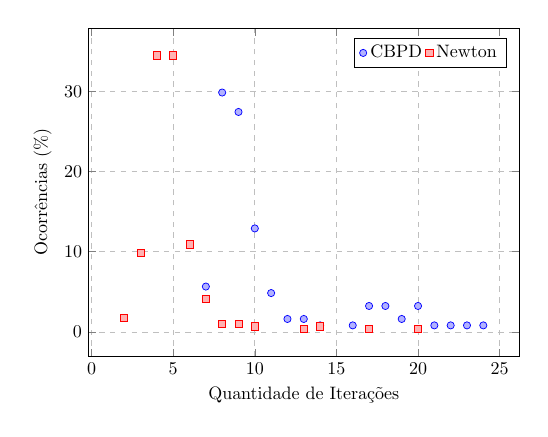
\begin{tikzpicture}[scale = 0.65]
  \begin{axis}[
    width=10cm,
    height=8cm,
    xlabel={Quantidade de Iterações},
    ylabel={Ocorrências (\%)},
    legend style={at={(0.5,-0.2)}, anchor=north, legend columns=-1},
    grid=major,
    grid style=dashed,
    legend pos=north east
  ]

    % First set of data
    \addplot[
      only marks,
      mark=*,
      color=blue,
      fill=blue!30,
    ] coordinates {
        (9, 27.42)
        (10, 12.90)
        (8, 29.84)
        (7, 5.65)
        (11, 4.84)
        (13, 1.61)
        (12, 1.61)
        (18, 3.23)
        (20, 3.23)
        (23, 0.81)
        (24, 0.81)
        (22, 0.81)
        (17, 3.23)
        (19, 1.61)
        (14, 0.81)
        (21, 0.81)
        (16, 0.81)
      };

    % Second set of data
    \addplot[
      only marks,
      mark=square*,
      color=red,
      fill=red!30,
    ] coordinates {
        (4, 34.47)
        (5, 34.47)
        (3, 9.90)
        (2, 1.71)
        (6, 10.92)
        (8, 1.02)
        (7, 4.10)
        (10, 0.68)
        (17, 0.34)
        (13, 0.34)
        (9, 1.02)
        (14, 0.68)
        (20, 0.34)
    };
    \legend{CBPD, Newton}

  \end{axis}
\end{tikzpicture}
\end{center}
